
\documentclass[aspectratio=169]{beamer}
%-----------------------------------------------------------------------
%%%% packages y comandos personales %%%%
\usepackage[utf8]{inputenc}
\usepackage[spanish]{babel}
\usepackage{alltt}
\usepackage{hyperref}
\usepackage[Symbol]{upgreek}
\usepackage{latexsym} % S\'imbolos
\usepackage{amsmath,amssymb,amsfonts}
\usepackage{graphics,epsfig,subfigure}
\usepackage{url}
\usepackage{caption}
\usepackage{multimedia}
\usepackage{slashbox}
\usepackage{media9}
\usepackage[Symbol]{upgreek}
\usepackage{MnSymbol}
\usepackage{tikz}
\usepackage{palatino}
\usepackage{color}
\usepackage[skins,theorems]{tcolorbox}
\usepackage[Symbol]{upgreek}
\usepackage{MnSymbol}
\usepackage{geometry}
\usepackage{tabularx}
\usepackage{arydshln}
\usepackage{textcomp}
\usepackage{marvosym}
\usepackage{lipsum}
\usepackage{pifont}
\usepackage{algorithmic}
\usepackage{longtable}
\usepackage{lscape}
\usepackage{booktabs}
\usepackage{bm}
\usepackage{enumitem}
%-----------------------------------------------------------------------
\newtheorem{Teorema}{Teorema}
\newtheorem{Ejemplo}{Ejemplo}
\newtheorem{Definicion}{Definici\'on}
\newtheorem{Corolario}{Corolario}
\newtheorem{Prueba}{Prueba}
%-----------------------------------------------------------------------
\mode<presentation>
{
  \usetheme{Boadilla}      % try: Default, Boadilla, Darmstadt, Madrid, Warsaw, Montpellier ...
  \usecolortheme{whale} % try: whale albatross, beaver, crane, ...
  \usefonttheme{professionalfonts}  % intente serif, structurebold, ...
  \setbeamertemplate{navigation symbols}{}
  \setbeamertemplate{caption}[numbered]
  \usefonttheme{serif}
  \setbeamertemplate{blocks}[rounded][shadow=true]
}
%-----------------------------------------------------------------------
\title[TP0]{Desarrollo del TP0: Atrapando Pokemons}
\author[Grupo ITBA No.]{Mauro Baquero-Su\'arez \inst{1} \and Dario Alejandro Peñaloza \inst{1} \and Lucas Miguel Biolley \inst{1} \and Marian... \inst{1}}
\institute[ITBA]{\inst{1} Instituto Tecnológico de Buenos Aires (ITBA)}
\date[\today]{
\includegraphics[scale=.034]{Figures/ITBA_Logo.png}}
%-----------------------------------------------------------------------
% Define colors:
\definecolor{JadeGreen}{RGB}{0,128,168}
\definecolor{ParakeetGreen}{RGB}{34,177,76}
\definecolor{UBCblue}{rgb}{0.04706, 0.15725, 0.296667} % UBC Blue (primary)
\definecolor{UBCgrey}{rgb}{0.3686, 0.5255, 0.6235} % UBC Grey (secondary)
% Beamer colors:
\setbeamercolor{palette primary}{bg=UBCblue,fg=white}
\setbeamercolor{palette secondary}{bg=UBCgrey,fg=white}
\setbeamercolor{palette tertiary}{bg=UBCblue,fg=white}
\setbeamercolor{palette quaternary}{bg=UBCblue,fg=white}
\setbeamercolor{structure}{fg=UBCblue} % itemize, enumerate, etc
\setbeamercolor{section in toc}{fg=UBCblue} % TOC sections
% Override palette coloring with secondary
\setbeamercolor{subsection in head/foot}{bg=UBCgrey,fg=white}
% Color boxes:
\tcbset{myinner/.style={no shadow,shrink tight,extrude by=1mm,colframe=blue,colback=blue!5!white,
  boxrule=0.6pt,frame style={opacity=0.25},interior style={opacity=0.5}}}
%-----------------------------------------------------------------------
\begin{document}
\spanishdecimal{.}
\maketitle
%-----------------------------------------------------------------------
\section{Introducción}
%-----------------------------------------------------------------------
\begin{frame}
\frametitle{Introducción}
El objetivo de este TP es evaluar una función que depende de varios parámetros de entrada, fundamentando las conclusiones con gráficos pertinentes y explicando la metodología utilizada para llegar a cada una. Para ello será provisto un código fuente que incluye una implementación de dicha función junto con ejemplos de ejecución.
\end{frame}
%-----------------------------------------------------------------------
\section{Desarrollo de las Preguntas}
%-----------------------------------------------------------------------
\begin{frame}
\frametitle{Pregunta No. 1: Acerca de las Pokebolas}
\begin{enumerate}[label=\emph{\alph*}), series=l_after]
\item Ejecutando la función 100 veces, para cada Pokemon en condiciones ideales (HP:100\%, LVL 100) ¿Cuál es la probabilidad de captura promedio para cada Pokebola?
\end{enumerate}
\end{frame}
%-----------------------------------------------------------------------
\begin{frame}
\frametitle{Pregunta No. 1: Acerca de las Pokebolas}
\framesubtitle{Respuesta a la pregunta}
\begin{center}
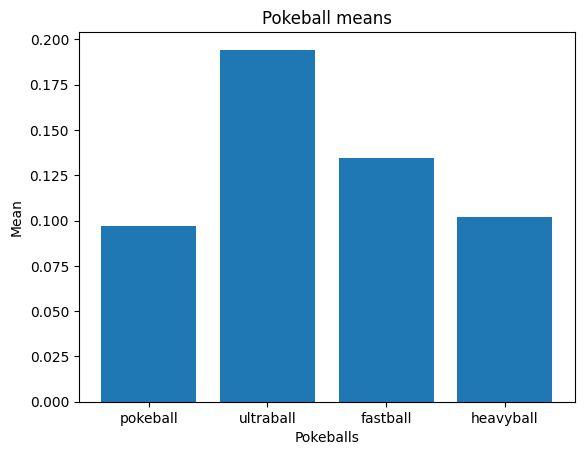
\includegraphics[scale=.35]{Figures/output_1a.png}
\end{center}

\vspace{-.5cm}
\begin{itemize}
\item En general las ultraball tienen mayor promedio de probabilidad de captura.
\item Las Ultraball tienen en general una probabilidad muy baja (Casi un 20\%).
\item Para tener éxito en la captura de un pokemon, se debe debilitar u optar por alguna otra criatura con un nivel de experiencia bajo.
\end{itemize}
\end{frame}
%-----------------------------------------------------------------------
\begin{frame}
\frametitle{Pregunta No. 1: Acerca de las Pokebolas}
\begin{enumerate}[label=\emph{\alph*}), resume*=l_after]
\item ¿Es cierto que algunas pokebolas son más o menos efectivas dependiendo de propiedades intrínsecas de cada Pokemon? Justificar.

\vspace{.5mm}
Sugerencia: Comparar efectividad (success/total attemps) como proporción de la efectividad de la Pokebola básica para cada Pokemon.
\end{enumerate}
\end{frame}
%-----------------------------------------------------------------------
\begin{frame}
\frametitle{Pregunta No. 1: Acerca de las Pokebolas}
\framesubtitle{Respuesta a la pregunta}

\begin{columns}
\column{.45\textwidth}
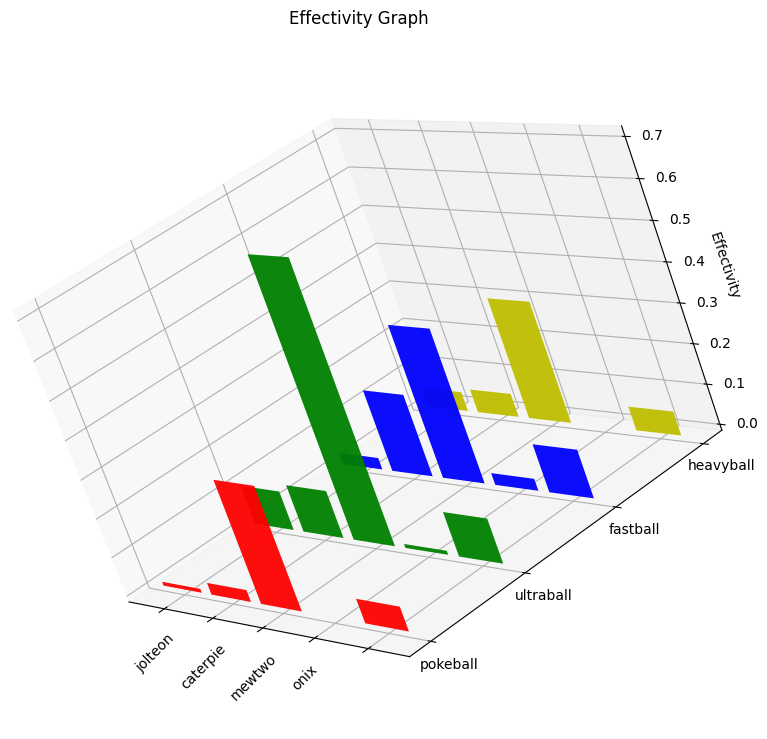
\includegraphics[scale=.352]{Figures/output_1b.png}
\column{.55\textwidth}
\begin{itemize}
\item La efectividad del tipo de pokebola si depende del pokemon a capturar.
\item Con las Ultraball se obtiene una efectividad del 65\% con pokemons no tan fuertes, sin necesidad de debilitarlos.
\item Mewtwo es muy dificil de capturar independientemente de la pokebola que se use.
\item Las Fastball son las más efectivas para pokemon rápido tipo rayo, como Jolteon.
\end{itemize}
\end{columns}
\end{frame}
%-----------------------------------------------------------------------
\begin{frame}
\frametitle{Pregunta No. 2: Acerca del estado del Pokemon}

\begin{enumerate}[label=\emph{\alph*}), series=l_after]
\item ¿Las condiciones de salud tienen algún efecto sobre la efectividad de la captura? Si
es así, ¿Cuál es más o menos efectiva?
\end{enumerate}
\end{frame}
%-----------------------------------------------------------------------
\begin{frame}
\frametitle{Pregunta No. 2: Acerca del estado del Pokemon}

\begin{enumerate}[label=\emph{\alph*}), resume*=l_after]
\item ¿Cómo afectan los puntos de vida a la efectividad de la captura?

\vspace{.5mm}
Sugerencia: Elegir uno o dos Pokemones y manteniendo el resto de los parámetros constantes, calcular la probabilidad de captura para distintos HP \%.
\end{enumerate}
\end{frame}
%-----------------------------------------------------------------------
\begin{frame}
\frametitle{Pregunta No. 2: Acerca del estado del Pokemon}

\begin{enumerate}[label=\emph{\alph*}), resume*=l_after]
\item ¿Qué parémetros son los que más afectan la probabilidad de captura?
\end{enumerate}
\end{frame}
%-----------------------------------------------------------------------
\begin{frame}
\frametitle{Pregunta No. 2: Acerca del estado del Pokemon}

\begin{enumerate}[label=\emph{\alph*}), resume*=l_after]
\item Teniendo en cuenta uno o dos pokemones distintos: ¿Qué combinación de condiciones (propiedades mutables) y pokebola conviene utilizar para capturarlos?
\end{enumerate}
\end{frame}
%-----------------------------------------------------------------------
\begin{frame}
\frametitle{Pregunta No. 2: Acerca del estado del Pokemon}

\begin{enumerate}[label=\emph{\alph*}), resume*=l_after]
\item  A partir del punto anterior, ¿sería efectiva otra combinación de parámetros teniendo en cuenta un nivel del pokemon más bajo (o más alto)?
\end{enumerate}
\end{frame}
%-----------------------------------------------------------------------
\section{Conclusiones}
%-----------------------------------------------------------------------
\begin{frame}
\frametitle{Conclusiones}
\begin{itemize}
\item ....\vspace{.25cm}
\item ....
\end{itemize}
\end{frame}
%-----------------------------------------------------------------------
\begin{frame}
\frametitle{Final de la presentación}

\Huge Gracias...!
\end{frame}
%-----------------------------------------------------------------------
\end{document}